%%%%%%%%%%%%%%%%%%%%%%% file template.tex %%%%%%%%%%%%%%%%%%%%%%%%%
%
% This is a general template file for the LaTeX package SVJour3
% for Springer journals.          Springer Heidelberg 2010/09/16
%
% Copy it to a new file with a new name and use it as the basis
% for your article. Delete % signs as needed.
%
% This template includes a few options for different layouts and
% content for various journals. Please consult a previous issue of
% your journal as needed.
%
%%%%%%%%%%%%%%%%%%%%%%%%%%%%%%%%%%%%%%%%%%%%%%%%%%%%%%%%%%%%%%%%%%%
%
% First comes an example EPS file -- just ignore it and
% proceed on the \documentclass line
% your LaTeX will extract the file if required
% \begin{filecontents*}{example.eps}
% %!PS-Adobe-3.0 EPSF-3.0
% %%BoundingBox: 19 19 221 221
% %%CreationDate: Mon Sep 29 1997
% %%Creator: programmed by hand (JK)
% %%EndComments
% gsave
% newpath
%   20 20 moveto
%   20 220 lineto
%   220 220 lineto
%   220 20 lineto
% closepath
% 2 setlinewidth
% gsave
%   .4 setgray fill
% grestore
% stroke
% grestore
% \end{filecontents*}
%
\RequirePackage{fix-cm}
%
%\documentclass{svjour3}                     % onecolumn (standard format)
%\documentclass[smallcondensed]{svjour3}     % onecolumn (ditto)
\documentclass[smallextended]{svjour3}       % onecolumn (second format)
%\documentclass[twocolumn]{svjour3}          % twocolumn
%
\smartqed  % flush right qed marks, e.g. at end of proof
%

\usepackage{amsmath}

\usepackage{graphicx}
\def\gfxdir{./gfx/}


% FIXME: REMOVE BEFORE SUBMITTING!
\usepackage{comment}
\usepackage{color}

%
% \usepackage{mathptmx}      % use Times fonts if available on your TeX system
%
% insert here the call for the packages your document requires
%\usepackage{latexsym}
% etc.
%
% please place your own definitions here and don't use \def but
% \newcommand{}{}
%
% Insert the name of "your journal" with
% \journalname{myjournal}
%
\begin{document}

\title{Direct and Inverse Dynamics Analysis of the Human Spine for
       Helicopter-Pilot Interaction}
%about the article that should go on the front page should be
%placed here. General acknowledgments should be placed at the end of the article.}
% \subtitle{Do you have a subtitle?\\ If so, write it here}

%\titlerunning{Short form of title}        % if too long for running head

\author{Andrea Zanoni,
        Alessandro Cocco
        and
	    Pierangelo Masarati%etc.
}

%\authorrunning{Short form of author list} % if too long for running head

\institute{A. Zanoni \at
              Department of Aerospace Science and Technology,
	      Politecnico di Milano, Milano, Italy\\
              Tel.: +39-02-23998035\\
              \email{andrea.zanoni@polimi.com}           %  \\
%             \emph{Present address:} of F. Author  %  if needed
	   ,
           A. Cocco \at
              Department of Aerospace Science and Technology,
	      Politecnico di Milano, Milano, Italy\\
              \email{alessandro.cocco@polimi.com}           %  \\
           P. Masarati \at
              Department of Aerospace Science and Technology,
	      Politecnico di Milano, Milano, Italy\\
              \email{pierangelo.masarati@polimi.com}           %  \\
}

\date{Received: date / Accepted: date}
% The correct dates will be entered by the editor


\maketitle

\begin{abstract}
Insert your abstract here. Include keywords, PACS and mathematical
subject classification numbers as needed.
\keywords{First keyword \and Second keyword \and More}
% \PACS{PACS code1 \and PACS code2 \and more}
% \subclass{MSC code1 \and MSC code2 \and more}
\end{abstract}

\section{Introduction}
\label{sec:intro}
The vibrational response of the human body is directly related to unpleasant sensations
(discomfort), degradation of efficiency in performing a task and may ultimately lead to
health related issues~\cite{griffin-1996-hbhv,garg-1976-ie3tsmc,hill-2009-jb}.
Thus, proper modeling of the human body response is of critical importance when evaluating
both vehicle comfort performance~\cite{deoliveira-2005-asem} and potential adverse
involuntary feedthrough of command inputs~\cite{quaranta-2013-jsv}, especially when,
as is the case in rotorcraft, they exhibit an intrinsic propensity to develop a high level
of vibrations.

Parameters of the vibratory response of the human body depend on its mechanical properties
and geometry, which in turn may depend on anthropometric
variables like age, gender, weight and stature. Therefore, the variance of the parameters
influencing the response has to be taken into account in the design stage, in order to
ensure an adequate level of robustness. Multibody modeling is a viable tool in this
context, since it can be viewed as first-principles approach. Starting from the
anthropometric parameters, through the geometrical and structural modeling, it supports the
extraction of the relevant synthetic parameters evaluating the fitness of a particular
design choice to the goal of achieving a greater pilot (or passenger) comfort
and/or of reducing the insurgence of possible triggers of adverse interaction
phenomena. 

This work is specifically focused on the multibody modeling of the human spine. A complete
model able to comprehend the spine behaviour has been developed in the
free general purpose multibody solver MBDyn, aimed at direct and inverse dynamics analyses,
and reduced order model extraction. Although at the current stage the model is
primarily used to estimate properties related to spine vertical dynamics in the
sagittal plane, it easy to reconfigure it to capture the full 3-dimensional
behavior of the spine.

As stated in the previous paragraphs, the model is aimed especially to
comfort-related modeling of rotorcraft. In this context, one of the most
important measures is the total force transmissibility between the human subject
(i.e. the pilot or the passenger of the analyzed rotorcraft) and the rotorcraft
itself. Therefore, a comparison between experimental data available in the
literature and the model results in terms of the mechanical impedance at the
interface point between the body and the seat has been carried out. \\
\textcolor{red}{TODO: completare}


\section{Human spine multibody model}\label{sec:mbdmodel}
% Figure
\begin{figure}[htbp]
  \centering
  \hfil
  \includegraphics[width=.171\textwidth]{\gfxdir spine_arms.png}
  \hfil
  \def\svgwidth{.3\textwidth}
  \input{\gfxdir vert_constr.eps_tex}
  \hfil
  \def\svgwidth{.3\textwidth}
  \input{\gfxdir vert_visc_constr.eps_tex} 
  \hfil
  \caption{Algebraic and deformable constraints connecting vertebr\ae\ nodes, indicated with
    	$V$, and viscer\ae\ nodes, indicated with $S$.}
  \label{fig:example}
\end{figure}

The model comprises 34 rigid bodies associated with nodes (i.e.\ entities
possessing degrees of freedom) placed in correspondence of vertebr\ae\ from S1 to C1, the
head, and of 8 visceral masses elastically connected to vertebr\ae\ from S1 to T10.
It follows the concepts proposed by Kitazaki and Griffin~\cite{KITAZAKI1997},
but extends the modeling to a full 3D representation of the upper body dynamics,
exploiting the database provided by Privitzer and
Belytschko~\cite{BELYTSCHKO-1978-AF-33615-76-C-0506}, whose sagittal plane data
was also used by Kitazaki and Griffin. 

Each vertebral section node is located in the center of the corresponding
vertebra's body, with axis $z$ aligned with the local tangent to the curve
described by the spine longitudinal axis, axis $y$ directed laterally and axis
$x$ pointing anteriorly (Cf. Fig.~\ref{fig:vertebra_RF}).

\begin{figure}[htbp]
	\centering
	\includegraphics[width=.3\textwidth]{\gfxdir vertebra_RF.png}
	\caption{Each node related to a vertebral section is located in the
	center of the corresponding vertebra's body, with axis $z$ along the
	local tangent to the spine axis curve and axis $y$ poiting laterally.
	\textcolor{red}{Figura non chiara: da rifare}}
	\label{fig:vertebra_RF}
\end{figure}

The spine itself is composed of 25 vertebral nodes connected by 24 linear
viscoelastic 3D elements, both acting on relative displacements and on relative
rotations between adjacent nodes. The head and the Sacrum are considered rigid
bodies and are also connected, respectively, to C1 and to L5 through a linear
viscoelastic elements. 

When restricted to the sagittal plane, vertebral nodes are connected to each other by
algebraic constraints limiting their relative degrees of freedom to sliding along the
spine axis and rotation about the lateral axis. When the model is used to perform
3-dimensional simulation, all of the vertebr\ae\ nodes relative rotation degrees of freedom
are unconstrained, while the translational constraints remain in place. 

Masses of viscerae, below the diaphram, are included as 8 additional rigid
bodies, connected to the corresponding vertebral nodes with linear viscoelastic
elements, as well.

The pelvic region is modeled taking into account the compliance of the buttocks
tissue, by introducing two viscoelastic elements connecting the Sacrum with a
node representing the mean interface point between the buttocks and the resting
surface.

Geometry and inertial parameters are adapted to represent a generic subject possessing
the desired anthropometric characteristics of age, gender, stature and weight,
as it will be described in detail in the next section.



\section{Human spine finite element model}
\label{sec:femmodel}
\input{femmodel}
\section{Model parametrization}\label{sec:parametrization}
The model target is represented by comfort-related simulations of the
vibrational response of the upper body of rotorcraft pilots and passengers. In
this context, the model should be able to reproduce the \emph{average}, or
\emph{most plausible} subject possessing a certain set of biometric
characteristics, whilst it it is not useful to build a purely subject-specific
model.   

The model is fully parametrized and can be generated starting from a generic
anthropometric dataset $\mathbf{s}$ comprising age, $a$, Body Mass Index
$\mathrm{BMI}$, stature $h$ and gender $g$:
\begin{equation}
	\mathbf{s} = \begin{bmatrix} a &\mathrm{BMI} &h &g \end{bmatrix}^{T}
	\label{eq:anthro_vect}
\end{equation}
A statistical model published by Shi et al.~\cite{SHI-2014-JB} is used to
generate the most plausible ribcage geometry associated with the anthropometric
parameters. The model of Shi et al. was derived from the analysis of thorax CT
scans of 89 subjects, divided in 8 age groups and of both sexes. Image
segmentation allowed to identify the position of 464 landmarks on the left side
of each subject's ribcage (Cfr. Fig.~\ref{fig:ribcage-3d}). The positions of the
landmarks were subjected to a PCA (Principal Component Analysis) following the
procedure outlined by Allen et al.\ in \cite{ALLEN-2003-ACMTC}. 

\begin{figure}[htbp]
	\centering
	\includegraphics[width=.8\textwidth]{\gfxdir ribcage}
	\caption{Example of the generated ribcage landmarks point cloud, using
	the model published by Shi et al.~\cite{SHI-2014-JB}. Values on the axes
	are in mm.}
	\label{fig:ribcage-3d}
\end{figure}

After generating the ribcage landmarks, a bounding box is fitted to them and its
dimensions $x, y, z$ are compared to those of the reference subject used in the
work of Kitazaki and Griffin~\cite{KITAZAKI1997} to yield three scaling
coefficients:
\begin{subequations}
	\begin{align}
		\lambda_x &= \dfrac{x}{x_0} &\lambda_y &= \dfrac{y}{y_0}
		&\lambda_z &= \dfrac{z}{z_0}
	\end{align}
	\label{eq:scalingf}
\end{subequations}
Since~\cite{KITAZAKI1997} does not report the anthropometric characteristics of
the subject, they were estimated a-posteriori by searching through an Sequential
Quadratic Programming optimisation algorithm the set $\mathbf{s}_0$ that
minimises the mean square error of the distances between the estimated
landmarks, obtained through the ribcage model, closer to the vertebr\ae
transverse processes and their corresponding locations estimated from the data
of Kitazaki and Griffin. The resulting reference subject is a 34 years old male,
1.78 m tall and weighting 84 kilograms, for a BMI of approximately 26.5.

Using as reference the \emph{normal} configuration found
in~\cite{KITAZAKI1997}, the initial positions of nodes for the modelled subject
are obtained by directly scaling their components with the coefficients
$\lambda_i$.

Stiffnesses are instead scaled comparing them to \emph{equivalent} lumped axial
and bending stiffnesses as follows: 
\begin{subequations}
	\begin{align}
		K_a' \sim \dfrac{EA'}{L'} 
			& = \dfrac{EA\lambda_x\lambda_y}{L\lambda_z} 
	\end{align}
\end{subequations}

\subsection{Validation with experimental result}

\begin{table}[htbp]
  \centering
  
    \begin{tabular}{lllll}
    \textbf{Model} & \textbf{Age } & \textbf{Weight [Kg]} & \textbf{Stature [m]} & \textbf{BMI [kg/m\^2]} \\
    \hline
    \textbf{Min} & 33,7  & 54,88 & 1,591 & 21,681 \\
    \textbf{Mean} & 33,7  & 69,5  & 1,71  & 23,768 \\
    \textbf{Max} & 33,7  & 83,9  & 1,823 & 25,246 \\
    \end{tabular}%
    \caption{Antropometric parameters used for the comparison}
  \label{tab:addlabel}%
\end{table}%



\begin{figure}[htbp]
	\centering
	\includegraphics[width=\textwidth]{\gfxdir scaling-no-backrest}
	\caption{Comparison between the experimental apparent mass from \cite{TOWARD2011} and the FEM one}
	\label{fig:scaling-no-backrest}
\end{figure}

\begin{figure}[htbp]
	\centering
	\includegraphics[width=\textwidth]{\gfxdir frf_3_axis}
	\caption{Seat to head transmissibility in the three directions: comparison between experimental result of \cite{Mandapuram2012}
	\label{fig:frf_3}}
\end{figure}




\section{Solution strategies}\label{sec:solution}
The spine model has been developed aiming at a high level of generality in its
applications.  As an encompassing example, in the present work the solution
phases needed to extract a reduced order model (ROM) for the evaluation of the
upper body vertical vibration response of seated rotorcraft pilot/passengers
will be outlined. The general procedure consists in several simulation steps: 

\begin{enumerate}
  \item an underdetermined inverse kinematics analysis that determines the pose
    of the spine in relation with the imposed position of the head and of the
    buttocks;
  \vspace{-0.2em}
  \item an inverse dynamics analysis that estimates the passive muscular
    intervertebral moments;
    \vspace{-0.2em}
  \item a direct dynamics analysis aimed at estimating the effect of the active
    muscular intervertebral moments;
    \vspace{-0.2em}
  \item an eigenanalysis, directly performed on the system of Differential-Algebraic Equations (DAE) system, to extract the ROM.
\end{enumerate}

To obtain a square problem in the kinematic inversion when solving for the 
system's positions, a series of static problems are set up, in which \emph{dummy} springs
act on the redundant degrees of freedom \cite{IK:FumagalliASME}. The
stiffnesses of the springs act as penalty coefficients for the motion of the degrees of 
freedom they are connected to. They can, for example, be crafted to minimize the norm 
of the internal bending moment in the sagittal plane, due to weight.

From the inverse kinematics analysis, the configuration of maximum ergonomy 
of the spine is obtained. In the subsequent direct analysis, active muscular
moments are estimated introducing simple controllers that
introduce intervertebral axial forces and bending moments linearly proportional
to the difference between the current vertebr\ae\ relative positions and the 
maximum ergonomy configuration.

Once the equilibrium position has been reached, an eigenanalysis is performed 
to extract a ROM \cite{RIPEPI-2011} of the spine suitable for vibration analysis
in the vertical direction, to be used in linearized, 
comprehensive rotorcraft vibration analysis \cite{TAMER-2017-ERF}.
Alternatively, the complete multibody model can be used in direct multibody 
bioaeroservoelastic analysis of the system \cite{MASARATI-2015-ERF}.


\section{TO DO}
\begin{enumerate}
  \item completare descrizione sezione precedente (solution strategies) integrando
    materiale NDODYCON;
  \item aggiungere descrizione modello FEM + CMS;
  \item risultati vertical bounce braccio + spina;
  \item verificare scalatura:
    \begin{itemize}
      \item \textbf{masse}: imporre che massa totale della spina sia la frazione
	\emph{corretta} della massa totale del corpo (scalare con modello 3D ribcage solo
	la distribuzione??);
      \item \textbf{rigidezze intervertebrali}:
	\begin{align}
	  K_a &\propto \lambda_x \lambda_y \\ 
	  K_{b,x} &\propto \lambda_x \lambda_y^2 \\
	  K_{b,y} &\propto \lambda_x^2 \lambda_y
	\end{align}
      \item \textbf{rigidezze buttocks}: mantenere come adesso per assiale. Per
	laterale\dots Ci pensiamo.
    \end{itemize}
\end{enumerate}

\section{Conclusions}
     



\begin{comment}
\subsection{Subsection title}
\label{sec:2}
as required. Don't forget to give each section
and subsection a unique label (see Sect.~\ref{sec:1}).
\paragraph{Paragraph headings} Use paragraph headings as needed.
\begin{equation}
a^2+b^2=c^2
\end{equation}

% For one-column wide figures use
\begin{figure}
% Use the relevant command to insert your figure file.
% For example, with the graphicx package use
  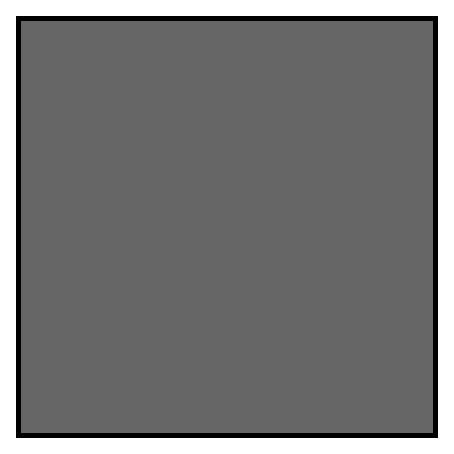
\includegraphics{example.eps}
% figure caption is below the figure
\caption{Please write your figure caption here}
\label{fig:1}       % Give a unique label
\end{figure}
%
% For two-column wide figures use
\begin{figure*}
% Use the relevant command to insert your figure file.
% For example, with the graphicx package use
  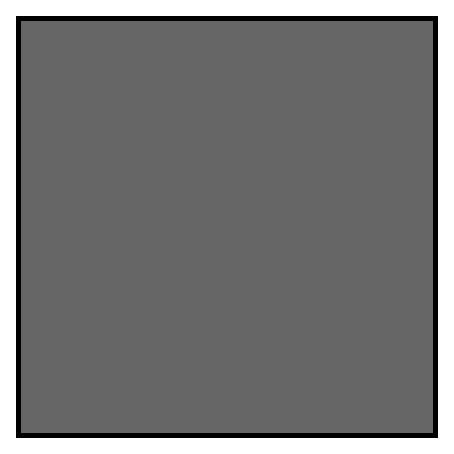
\includegraphics[width=0.75\textwidth]{example.eps}
% figure caption is below the figure
\caption{Please write your figure caption here}
\label{fig:2}       % Give a unique label
\end{figure*}
%
% For tables use
\begin{table}
% table caption is above the table
\caption{Please write your table caption here}
\label{tab:1}       % Give a unique label
% For LaTeX tables use
\begin{tabular}{lll}
\hline\noalign{\smallskip}
first & second & third  \\
\noalign{\smallskip}\hline\noalign{\smallskip}
number & number & number \\
number & number & number \\
\noalign{\smallskip}\hline
\end{tabular}
\end{table}
\end{template}
\end{comment}

%\begin{acknowledgements}
%If you'd like to thank anyone, place your comments here
%and remove the percent signs.
%\end{acknowledgements}

% BibTeX users please use one of
%\bibliographystyle{spbasic}      % basic style, author-year citations
\bibliographystyle{spmpsci}      % mathematics and physical sciences
%\bibliographystyle{spphys}       % APS-like style for physics
\bibliography{mybib,spine}   % name your BibTeX data base

% Non-BibTeX users please use
% \begin{thebibliography}{}
%
% and use \bibitem to create references. Consult the Instructions
% for authors for reference list style.
%
% \bibitem{RefJ}
% Format for Journal Reference
% Author, Article title, Journal, Volume, page numbers (year)
% Format for books
% \bibitem{RefB}
% Author, Book title, page numbers. Publisher, place (year)
% etc
% \end{thebibliography}

\end{document}
% end of file template.tex

